\documentclass[a4paper,12pt]{article}

% Pacotes necessários
\usepackage[utf8]{inputenc}
\usepackage[brazil]{babel}
\usepackage{hyperref}
\usepackage[T1]{fontenc}
\usepackage{graphicx}
\usepackage{caption}
\usepackage[left=2cm, right=2cm, top=2cm, bottom=2cm]{geometry}
\usepackage{lipsum} % Para gerar texto de preenchimento
\usepackage{float}
\usepackage{amsmath}
\usepackage{listings}
\usepackage{xcolor}


% Configuração da página de título
\newcommand{\reporttitle}{Trabalho 3 - Reator}
\newcommand{\reportauthor}{
Lucas William Junges}
\newcommand{\reportdate}{30/06/2025}
%\renewcommand{\listoffigures}{}
%\renewcommand{\tableofcontents}{}


\begin{document}

% Página de título personalizada
\begin{titlepage}
    \centering
    \vspace*{1cm}
    
\includegraphics[width=0.4\textwidth]{Imagens/BrasaoUFSC.png} % Adicione o caminho para o logotipo da sua instituição
    \par\vspace{1cm}
    {\scshape\Large Universidade Federal de Santa Catarina\par} % Substitua pelo nome da sua instituição
    \vspace{1.2cm}
    {\huge\bfseries \reporttitle\par}
    \vspace{2cm}
    {\Large\itshape \reportauthor\par}
    \vfill
    {\large \reportdate\par}
\end{titlepage}

% Lista de ilustrações
\listoffigures
\clearpage

% Sumário
\tableofcontents
\clearpage



\section{Introdução}

Na segunda parte deste estudo, foram desenvolvidas e implementadas técnicas avançadas de controle para um reator continuamente agitado, utilizado na produção de cyclopentenol (produto B) a partir de cyclopentadiene (produto A), com a presença de um catalisador diluído em água. O enfoque foi no projeto de um controlador utilizando a técnica de lugar de raízes, comparando seu desempenho com um controlador PI previamente desenvolvido. A análise incluiu simulações detalhadas do sistema não linear para verificar a robustez e eficácia dos controladores propostos.

Nesta terceira parte, o objetivo é enfrentar o desafio adicional de um atraso de medição na concentração de saída do produto B, que ocorre devido ao tempo de deslocamento do produto até o sensor e ao tempo de processamento do sensor, totalizando um atraso de 3 minutos. Este atraso exige um ajuste no sistema de controle da malha principal, desconsiderando as malhas internas e a ação feedforward estudadas anteriormente.

Para abordar este problema, será inicialmente projetado um controle baseado no Preditor de Smith em tempo discreto, visando manter as mesmas características transitórias (tempo de acomodação e pico máximo) e permanentes (erro em regime permanente) obtidas na parte 2. Este controlador deve garantir um ganho estático unitário na relação referência-saída de \(C_B\), utilizando um filtro de referência, se necessário. A eficácia do Preditor de Smith será avaliada por meio de simulações do modelo linearizado, com foco em respostas a degraus de referência de \(C_B\) e perturbações de \(C_{AF}\).

Serão realizadas simulações detalhadas do comportamento dinâmico do sistema com o modelo completo não linear utilizando o Simulink. As simulações incluirão cenários semelhantes aos da parte 2, com variações próximas ao ponto de operação e perturbações, para verificar se o sistema atende às especificações de desempenho e robustez. A resposta do sistema ao se afastar do ponto de operação será analisada, permitindo uma compreensão aprofundada da dinâmica do reator sob controle.

Além disso, será explorada a possibilidade de melhorar a resposta do Preditor de Smith utilizando uma versão filtrada deste controlador. A performance deste novo controle será comparada ao controle original, tanto em simulações do modelo linearizado quanto do modelo não linear. Esta análise permitirá avaliar se a inclusão do filtro melhora a resposta do sistema e contribui para uma maior robustez.

A análise incluirá a avaliação de robustez do sistema, a discussão dos resultados, a determinação do controle equivalente e a implementação por equações a diferença. Esta abordagem detalhada visa garantir que o sistema de controle proposto não apenas atenda às especificações iniciais, mas também seja capaz de manter desempenho consistente sob diferentes condições de operação.

O objetivo final desta parte do estudo é aprofundar o conhecimento sobre técnicas de controle avançadas aplicadas a sistemas com atraso. Utilizando o Preditor de Smith e sua versão filtrada, busca-se verificar a eficácia dessas abordagens em cenários realistas de operação através de simulações detalhadas. Esta investigação contribuirá para o desenvolvimento de estratégias de controle mais robustas e eficazes para processos químicos industriais.

\newpage

% Desenvolvimento
\section{Desenvolvimento}
\label{chap:desenvolvimento}

Na parte 2 se estudou o controle completo da concentração de produto em um reator 
continuamente agitado, usado na indústria química. Para este sistema foi estudada uma 
estrutura com uma malha interna e uma externa, assim como com ação feed fordward.
Para esta tarefa temos que estudar o mesmo problema da parte 2 (usando o mesmo ponto 
de equilíbrio e o mesmo modelo) mas considerando que na medida de concentração de saída 
B tem um atraso de 3 minutos causado pelo deslocamento do produto até o sensor e o tempo 
de processamento do sensor. Assim, neste caso, o sistema de controle da malha principal 
deveria ser reajustado. A malha interna de \(C_A\) ou o feedforward de \(C_{AF}\) não serão mais usadas 
aqui.

 \begin{figure}[ht]
  \centering
  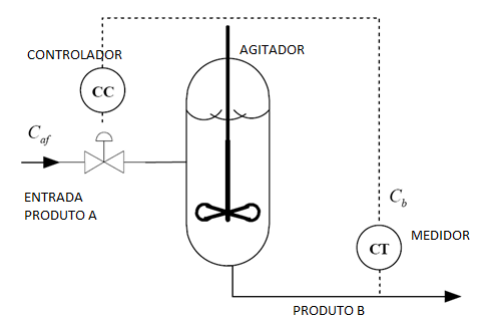
\includegraphics[width=0.6\textwidth]{Imagens/Reator.png}
  \caption{Reator químico}
  \end{figure}

\newpage

\section{Parte 3 -  Sistema de controle de um reator químico com atraso de medição de concentração}

\subsection{Projeto de Controle por Preditor de Smith}

a) Projete um controle com base no Preditor de Smith (em tempo discreto) para obter em malha fechada um sistema com aproximadamente as mesmas características transitórias (\(t_{5\%}\) e pico) e permanentes (erro em regime permanente) que as obtidas na parte 2 (considere o \(t_{5\%}\) medido depois do atraso). Essa especificação deve ser atendida para resposta a seguimentos de degraus de referência de \(C_B\) e perturbações de \(C_{AF}\). Use filtro de referência se necessário. Lembre-se que o sistema deve ter ganho estático unitário para a relação referência-saída de \(C_B\). Estude o comportamento do sistema sobre o modelo linearizado por simulação. Conclua sobre as propriedades em malha fechada do Preditor de Smith para este sistema. As especificações foram atendidas?\\

A primeira abordagem consiste na implementação do controle no sistema linearizado, incorporando um atraso de 3 minutos na leitura da concentração de \(C_B\). De acordo com as especificações, o controlador deve atender ao tempo de assentamento nas perturbações. Para alcançar este objetivo, será utilizada a estrutura do Preditor de Smith filtrado.

\begin{equation}
C_B = \frac{4.81}{(s+6.94)(s+1.64)}C_{AF} +\frac{-2.17(s-5.54)}{(s+6.94)(s+1.64)} U
\end{equation}

\begin{equation}
C_A = \frac{0.8}{(s+6.9433)}C_{AF} +\frac{4.5067}{s+6.9433} U
\end{equation}

Com as funções de transferência definidas, estas serão discretizadas utilizando o comando \texttt{c2d} do MATLAB. O período de amostragem utilizado (\(T_s\)) será de 0.07 segundo, conforme adotado na questão anterior.\\

\lstset{
  language=Octave,
  basicstyle=\ttfamily,
  keywordstyle=\color{blue},
  commentstyle=\color{gray},
  stringstyle=\color{red},
  showstringspaces=false,
  breaklines=true,
  frame=single,
  morekeywords={tf, c2d}
}


\begin{lstlisting}
clear;
clc;
close all;

% Definicao do sistema
s = tf('s');
ts = 0.07;

% Discretizacao de C_B
C_B_Caf = 4.81 / ((s + 6.94) * (s + 1.64));
C_B_U = -2.17 * (s - 5.54) / ((s + 6.94) * (s + 1.64));

C_B_Caf_discrete = c2d(C_B_Caf, ts, 'tustin');
C_B_U_discrete = c2d(C_B_U, ts, 'tustin');

% Discretizacao de Ca
Ca_Caf = 0.8 / (s + 6.9433);
Ca_U = 4.5067 / (s + 6.9433);

Ca_Caf_discrete = c2d(Ca_Caf, ts, 'tustin');
Ca_U_discrete = c2d(Ca_U, ts, 'tustin');

% Exibicao dos sistemas discretizados
C_B_Caf_discrete
C_B_U_discrete
Ca_Caf_discrete
Ca_U_discrete
\end{lstlisting}


Função de transferência \(C_B\)-\(C_{AF}\) discreta:\\

\begin{equation}
C_B(z): \quad \frac{0.004483 z^2 + 0.008967 z + 0.004483}{z^2 - 1.501 z + 0.543}C_{AF}(z)
\end{equation}\\

Tempo de amostragem: 0.07s\\

Função de transferência \(C_B\)-\(U\) discreta:

\begin{equation}
C_B: \quad \frac{-0.04658 z^2 + 0.02241 z + 0.069}{z^2 - 1.501 z + 0.543}U(z)
\end{equation}

Tempo de amostragem: 0.07s \\

Para o controlador do Preditor de Smith, será utilizado o controlador obtido na parte 2 por meio da técnica de lugar das raízes:

\begin{equation}
C(s) = \frac{0.93 s + 1.93}{s}
\end{equation}

O controlador pode ser discretizado usando a transformação de Tustin da seguinte forma:

Primeiro, substituímos \( s \) por \( \frac{2}{T} \cdot \frac{1 - z^{-1}}{1 + z^{-1}} \):

\[
C(z) = 0.93\left(\frac{\frac{2}{T} \cdot \frac{1 - z^{-1}}{1 + z^{-1}} + 2.07}{\frac{2}{T} \cdot \frac{1 - z^{-1}}{1 + z^{-1}}}\right)
\]\\

Simplificando, obtemos:

\[
C(z) = \frac{0.9928z - 0.8672}{z-1}
\]\\

Fazendo o sistema completo do Preditor de Smith em Simulink:

 \begin{figure}[H]
  \centering
  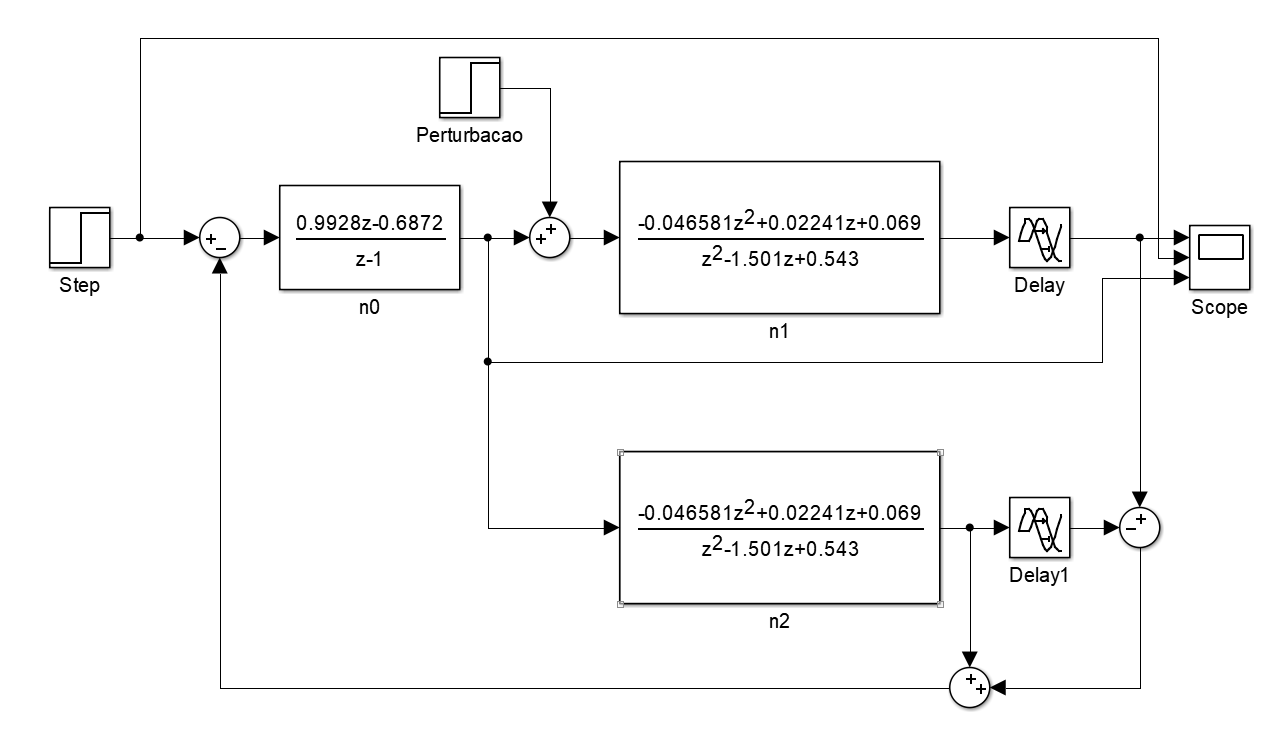
\includegraphics[width=0.9\textwidth]{Imagens/q1.png}
  \caption{Diagrama de Blocos do sistema discreto com Preditor de Smith}
  \end{figure}

  Obtêm-se a resposta ao degrau, entrada degrau e sinal de controle discreto, respectivamente:

   \begin{figure}[H]
  \centering
  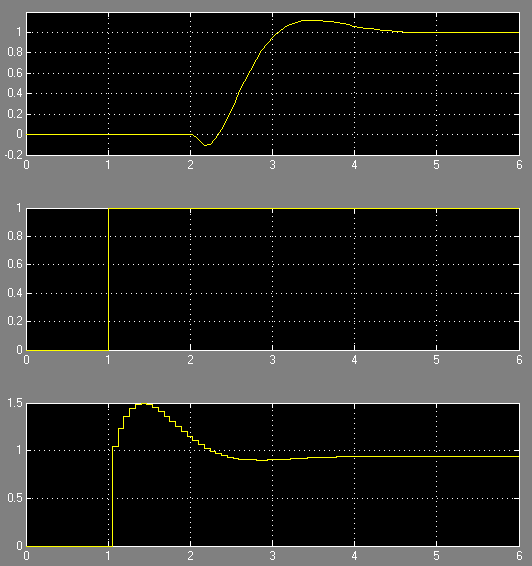
\includegraphics[width=0.75\textwidth]{Imagens/q12.png}
  \caption{Resposta ao degrau, entrada degrau e sinal de controle discreto}
  \end{figure}

  Com um atraso de 3 minutos considerado, o tempo de assentamento que obtivemos foi de 1,74 minuto, um valor muito próximo do esperado. No entanto, será necessário projetar um filtro de referência, pois o pico máximo alcançado excedeu o limite especificado na especificação (5 por cento de ultrapassagem). O filtro a ser projetado precisa cancelar os zeros dominantes presentes no controlador e assegurar um ganho unitário. Os requisitos para o filtro são os seguintes, baseado no controlador encontrado:

  \begin{align}
      C(z) = \frac{0.9928z -0.8672}{z-1}
  \end{align}

   \begin{align}
      Fr(z) = \frac{0.1256}{0.9928z-0.8672}
  \end{align}

  Assim, o diagrama de blocos com o filtro de referência incluso é:

 \begin{figure}[H]
  \centering
  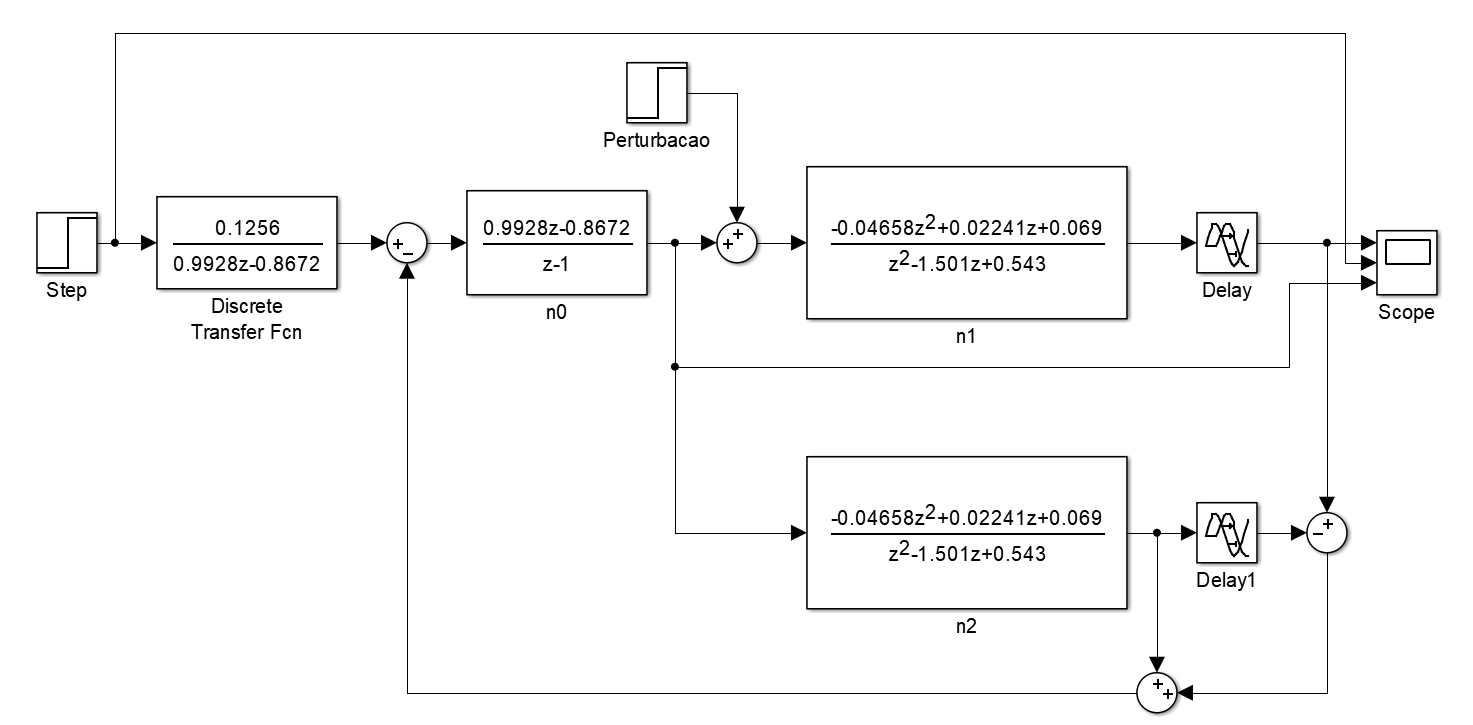
\includegraphics[width=0.95\textwidth]{Imagens/q11p.png}
  \caption{Diagrama de Blocos do sistema discreto com Preditor de Smith e Filtro de Referência}
  \end{figure}

E portanto a nova resposta ao degrau, entrada degrau e sinal de controle discreto, respectivamente é:

   \begin{figure}[H]
  \centering
  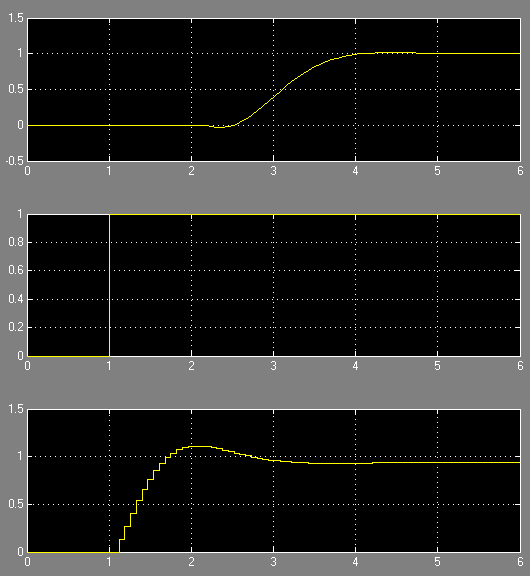
\includegraphics[width=0.75\textwidth]{Imagens/q13.png}
  \caption{Resposta ao degrau, entrada degrau e sinal de controle discreto com Filtro de Referência}
  \end{figure}

  Agora sim a resposta do sistema atende a todas as especificações exigidas. Para análise de perturbação do tipo degrau a resposta ao degrau, entrada degrau e sinal de controle discreto encontradas foram:

   \begin{figure}[H]
  \centering
  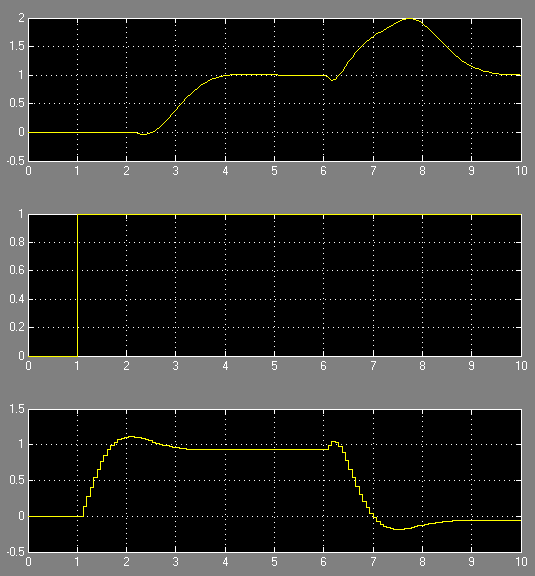
\includegraphics[width=0.82\textwidth]{Imagens/q1p.png}
  \caption{Resposta ao degrau perturbação, entrada degrau e sinal de controle discreto à perturbação com Filtro de Referência}
  \end{figure}

O resultado obtido em relação à perturbação foi aquém do desejado, o que se alinha com as expectativas, considerando que o controlador necessita de 3 segundos para detectar a perturbação e mais 3 segundos para reagir a ela. Adicionalmente, o Preditor de Smith funciona de maneira similar a um controlador de cancelamento, apresentando uma resposta inerentemente mais lenta para a rejeição de perturbações. A aplicação de filtros de predição pode ser uma alternativa para melhorar esse desempenho.

Com a utilização da estrutura do Preditor de Smith, as especificações para o controle da referência foram atendidas, porém as exigências relacionadas à rejeição de perturbações não foram plenamente alcançadas. As soluções potenciais para esta limitação serão exploradas nas próximas seções.

\newpage


  



\subsection{Simulação do comportamento dinâmico}

b) Usando Simulink, estude por simulação o comportamento dinâmico do sistema em malha fechada com o modelo completo não linear e verifique se atende as especificações. Utilize o mesmo cenário da parte 2, com a partida do sistema em rampa até chegar no ponto de operação e variações perto do ponto de operação, inclusive com perturbações. O que acontece com o sistema ao se afastar do ponto de operação? Realize um estudo de robustez para justificar os resultados.\\

Para analisar o funcionamento do controle com o preditor de Smith no sistema não linear, utilizamos um subsistema que inclui o modelo não linear alimentado por uma concentração constante de \(C_{AF}\) igual a 5.1. Esse subsistema foi integrado à estrutura do preditor de Smith.

\begin{figure}[H]
  \centering
  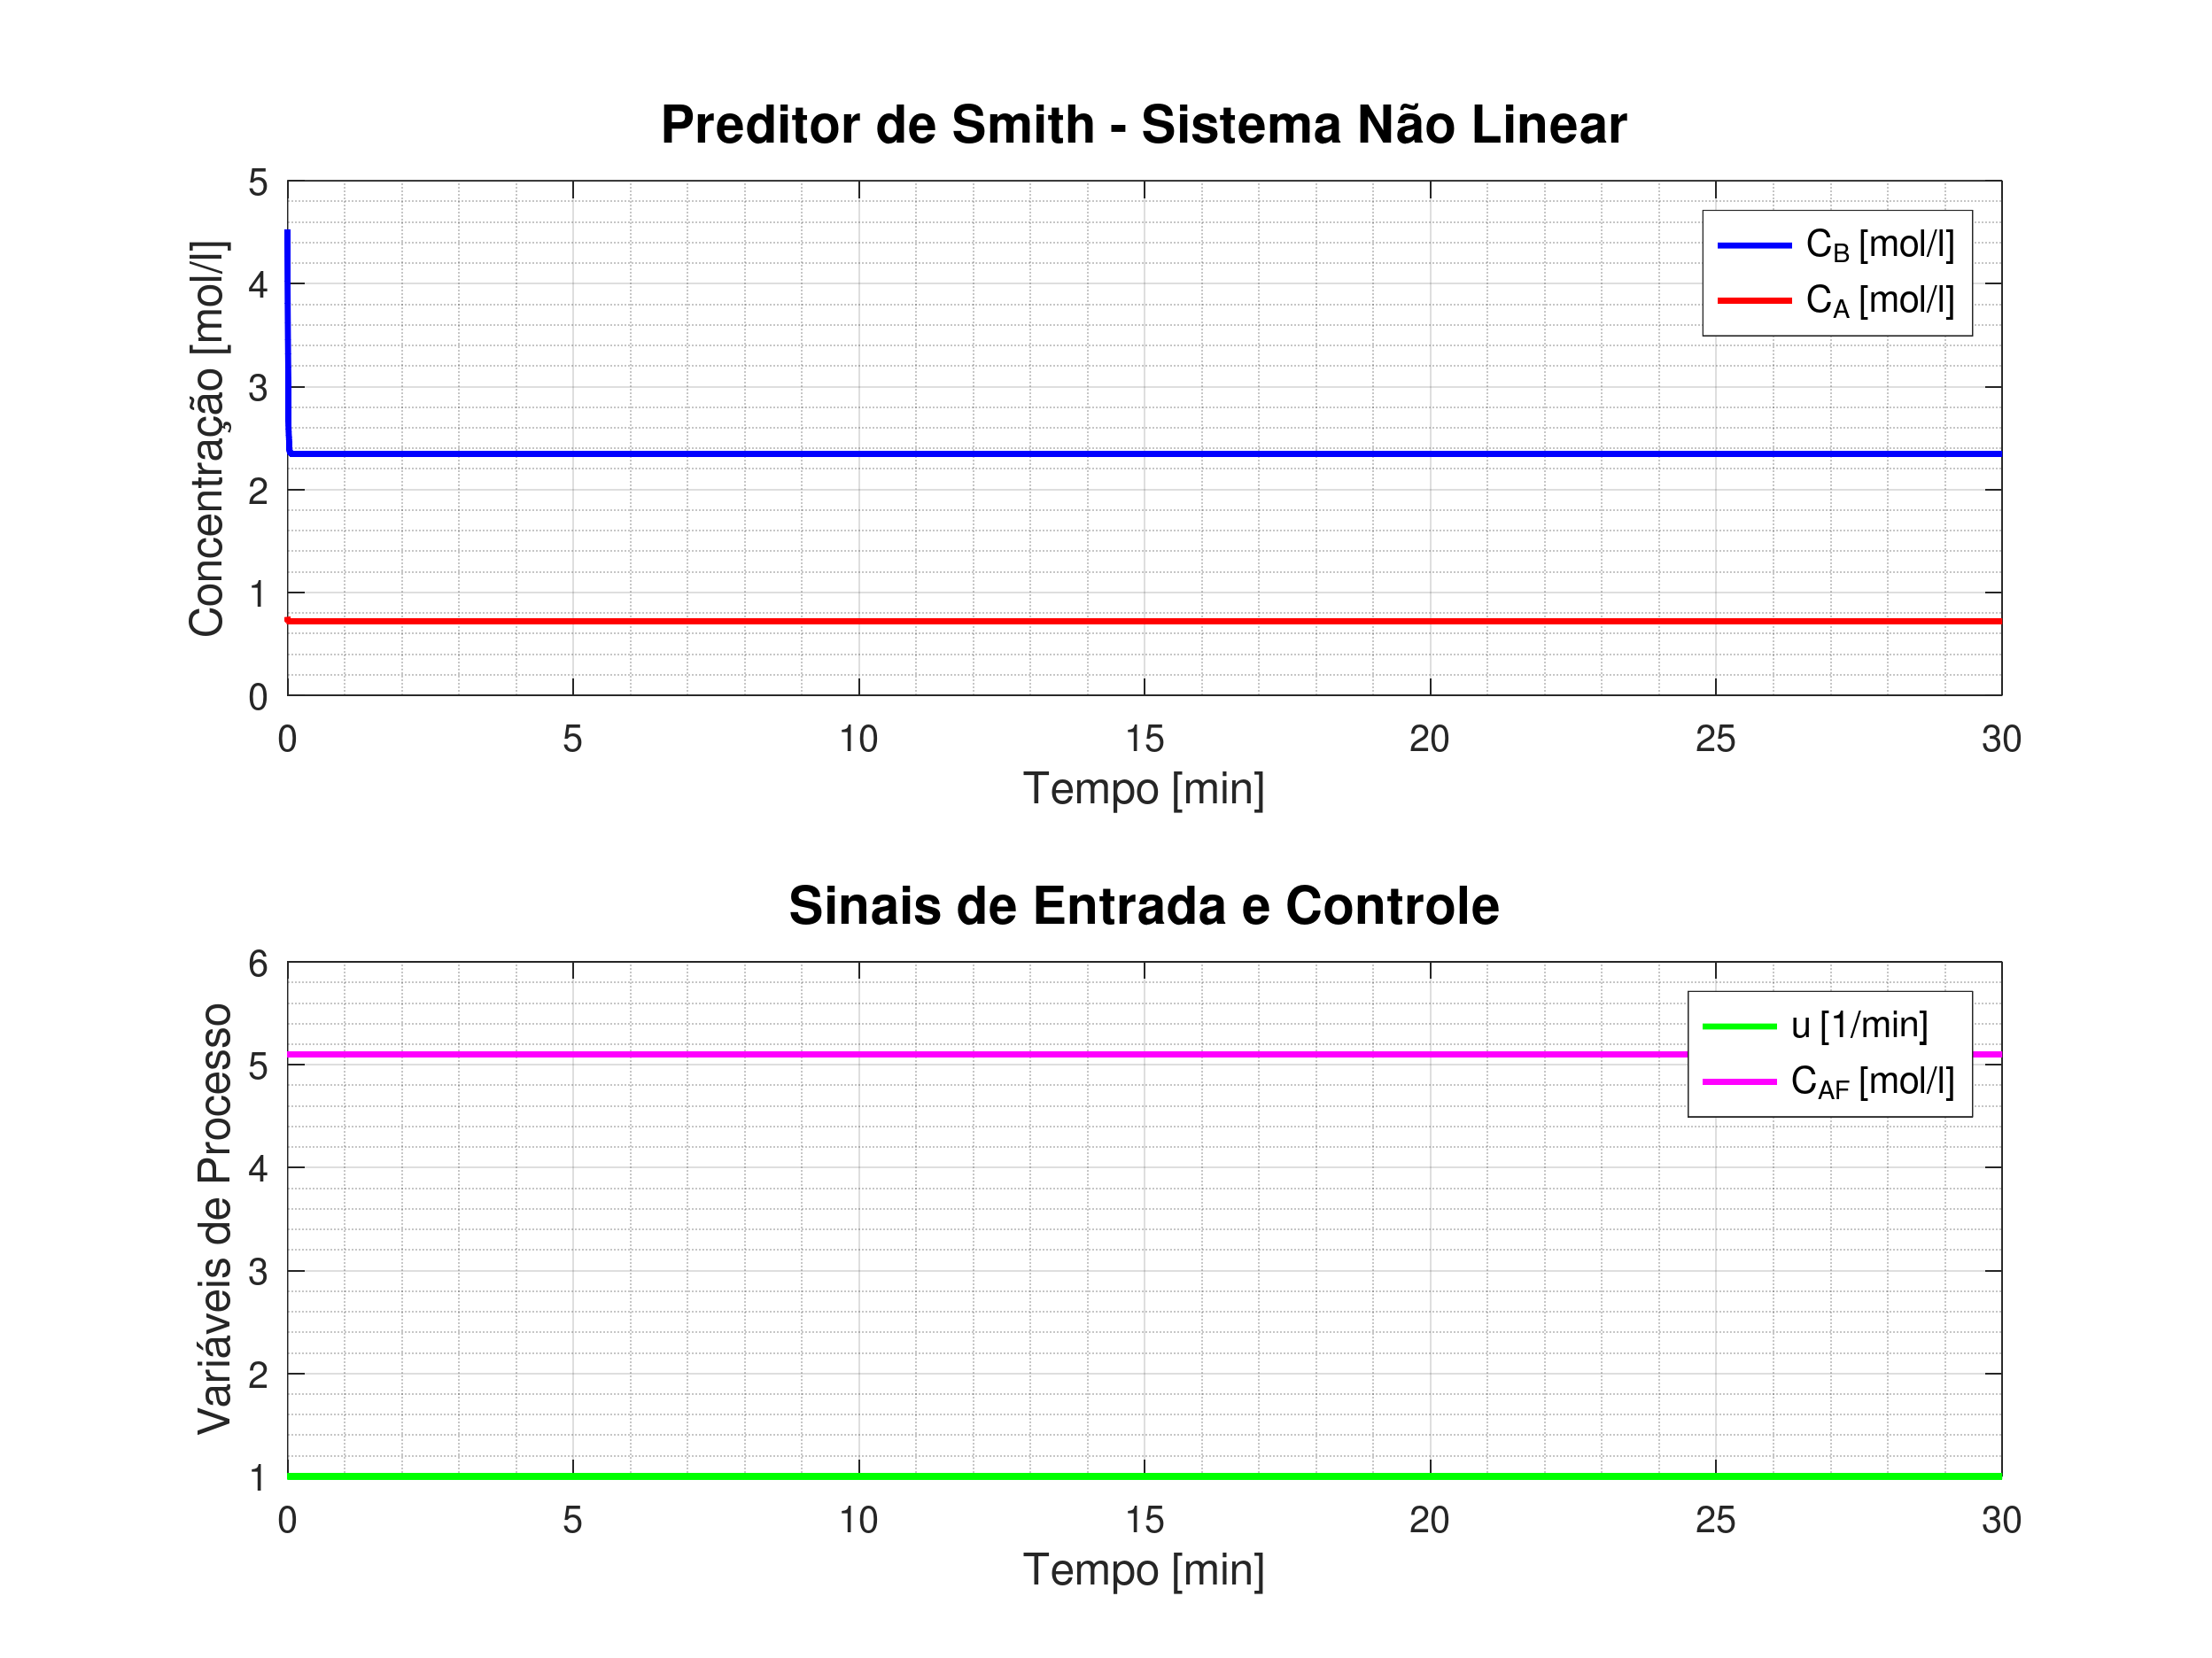
\includegraphics[width=0.82\textwidth]{figure5.png}
  \caption{Preditor de Smith com sistema não linear}
  \end{figure}

A resposta a mudanças de referência apresentou um tempo de aproximadamente 1.6 minutos, conforme ilustrado na figura abaixo.

\begin{figure}[H]
  \centering
  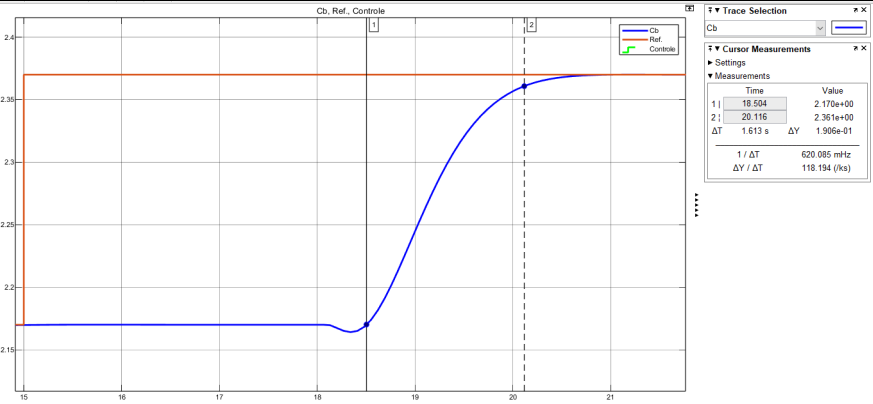
\includegraphics[width=0.82\textwidth]{figure6.png}
  \caption{Resposta Y/R no sistema não linear com mudanças do tipo degrau na referência}
  \end{figure}

Inserindo uma perturbação no tempo de 20 minutos com uma amplitude de -0.2 mol/l, observamos a seguinte rejeição da perturbação.

\begin{figure}[H]
  \centering
  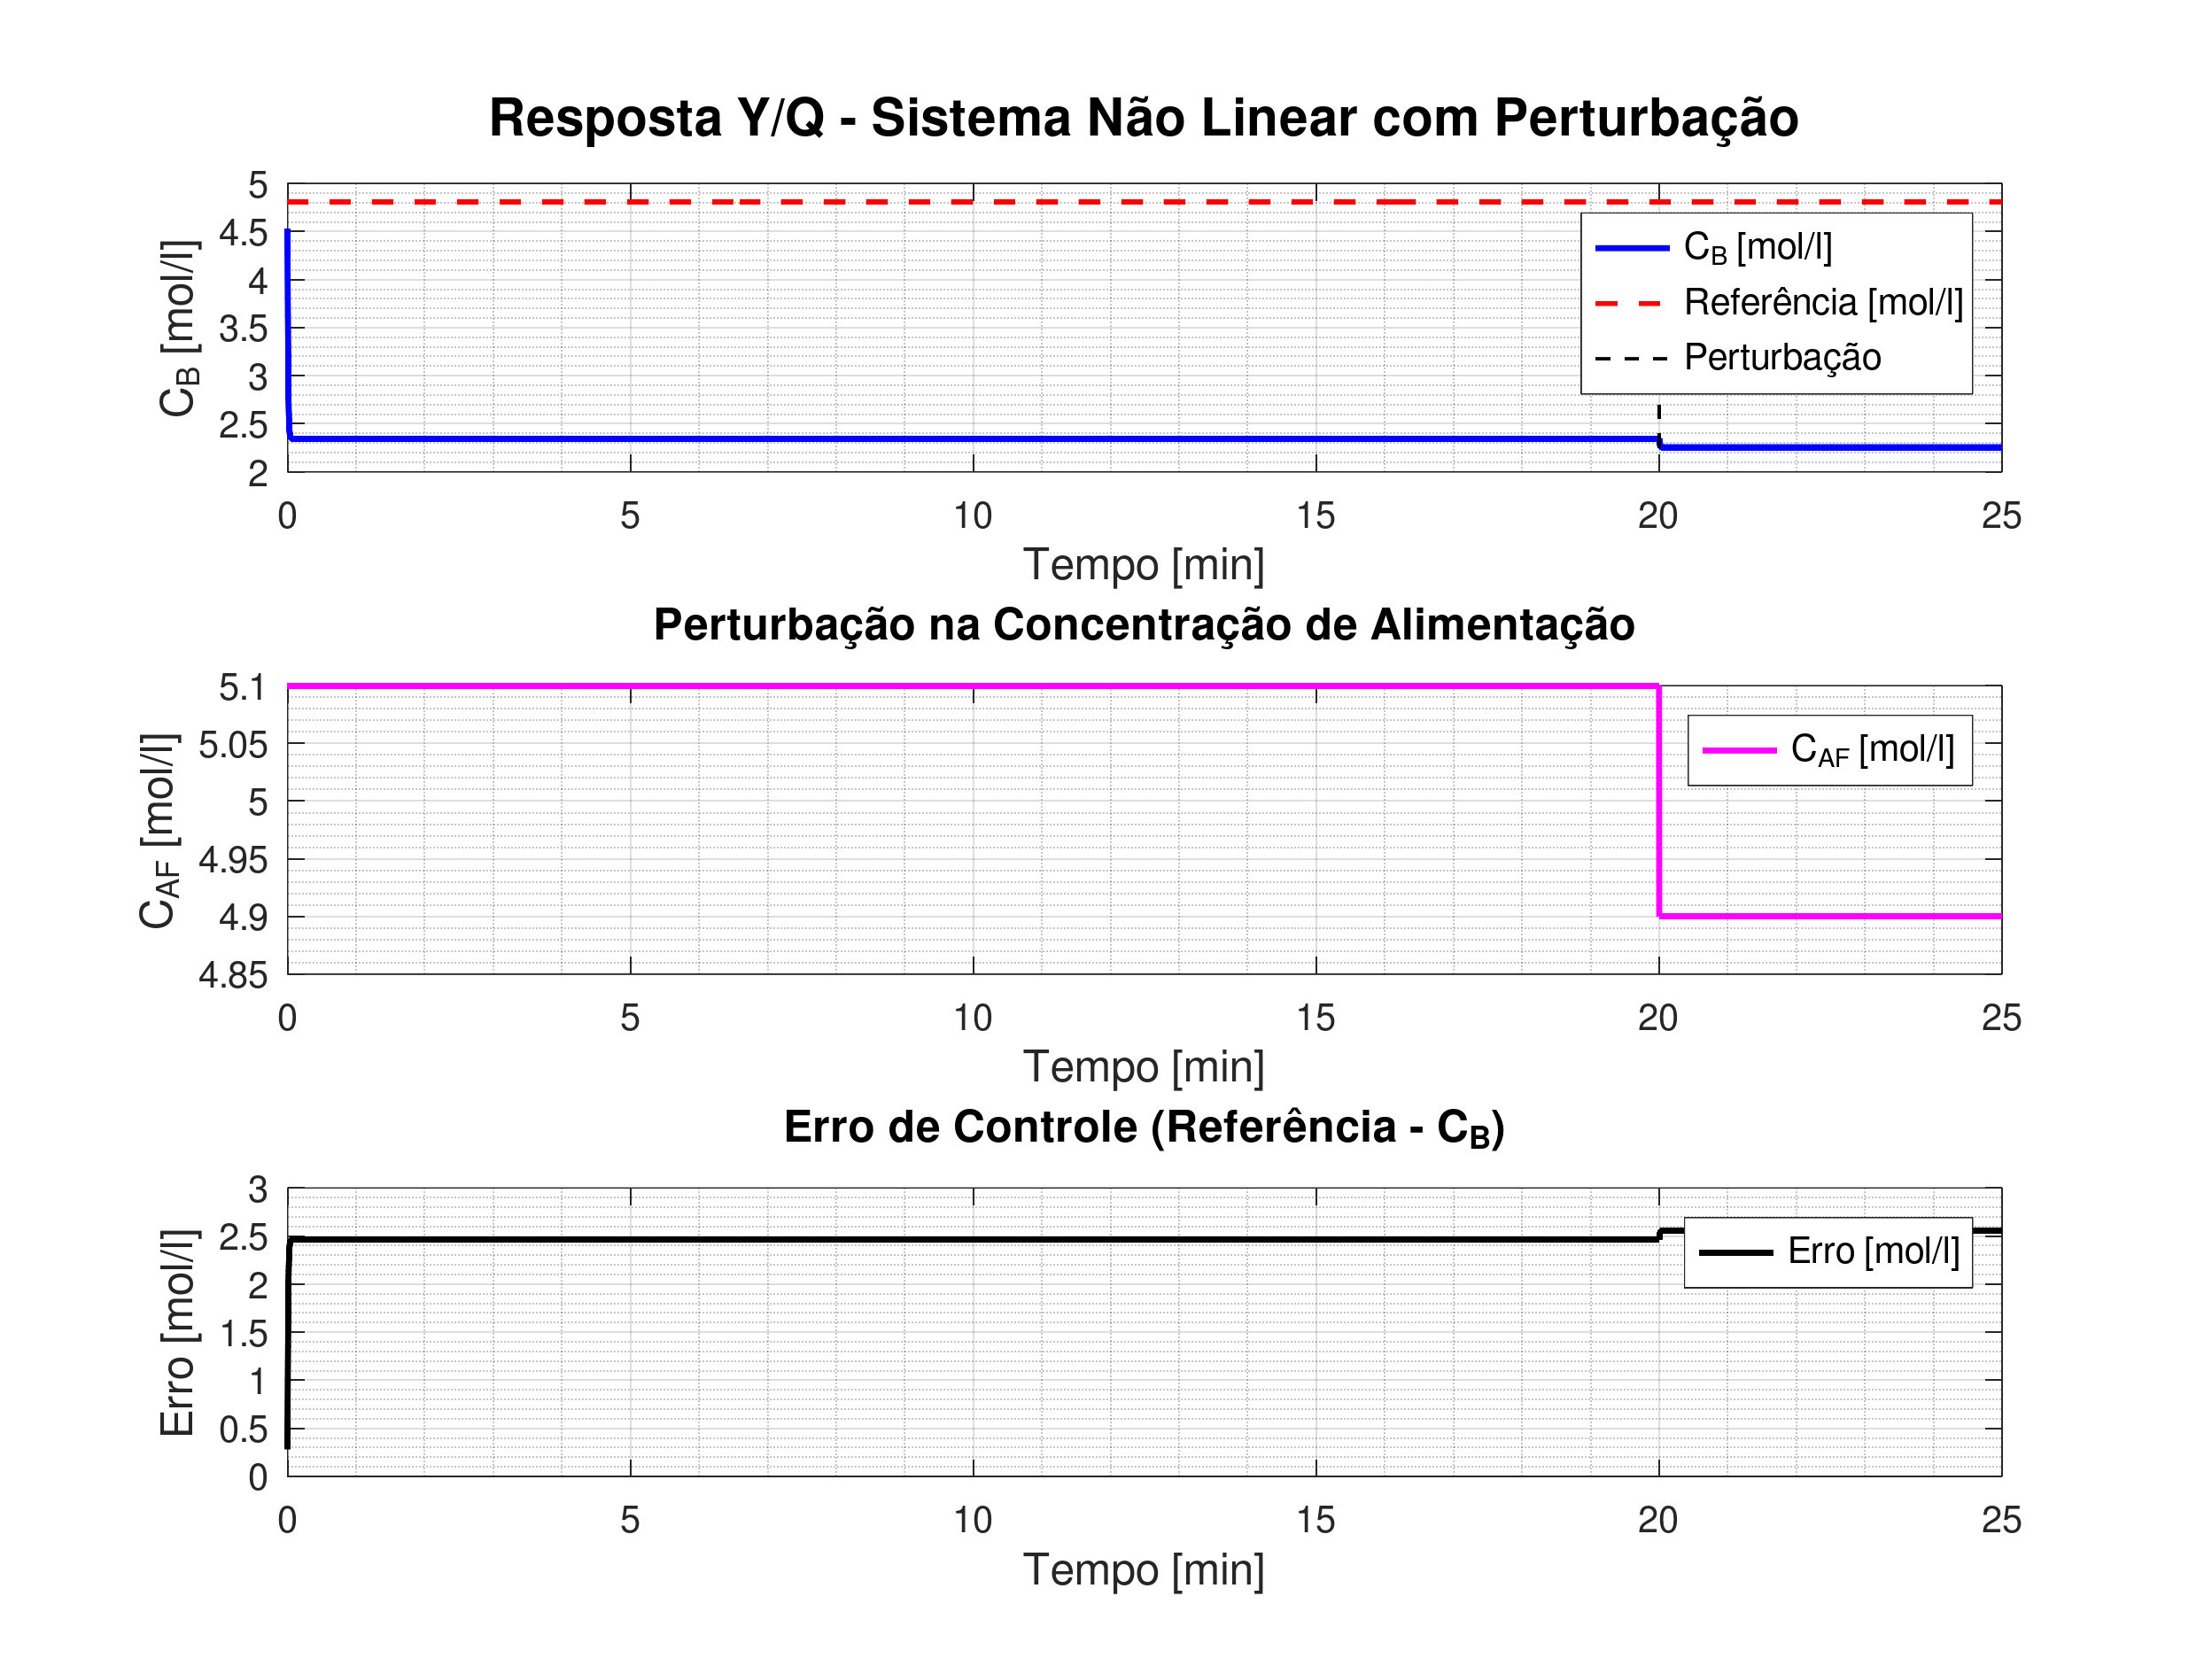
\includegraphics[width=0.82\textwidth]{figure7.png}
  \caption{Resposta Y/Q no sistema não linear com mudanças do tipo degrau na perturbação}
  \end{figure}

É possível notar que o tempo de rejeição das perturbações é satisfatório, embora ele aumente conforme a amplitude da perturbação se torna maior.

Próximo ao ponto de operação, o sistema de controle consegue estabilizar o sistema na referência desejada, mesmo com a inserção de perturbações. Vamos agora analisar grandes variações do ponto de operação.

Quando inserimos uma grande variação na referência, afastando-a consideravelmente do ponto de operação, verificamos que o sistema de controle não consegue fazer com que \(C_B\) atinja o valor de referência.

\begin{figure}[H]
  \centering
  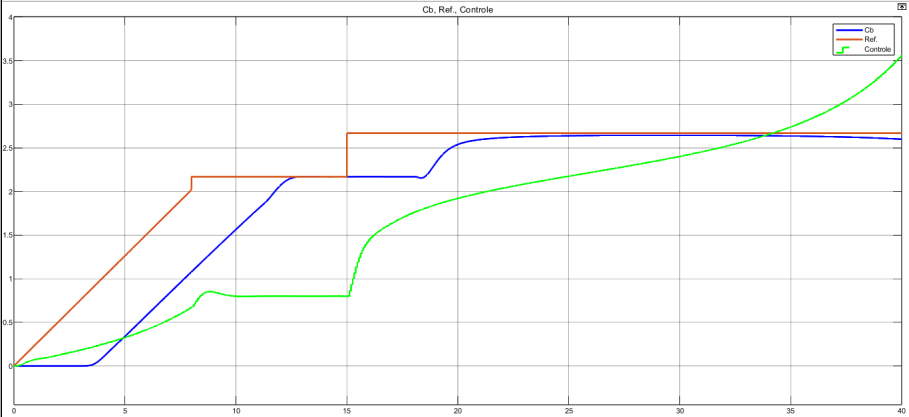
\includegraphics[width=0.82\textwidth]{figure8.png}
  \caption{Variação Grande de Referência}
  \end{figure}

Podemos concluir que o preditor de Smith apresenta certa robustez. Comparando com a parte 2, a variação máxima do ponto de operação que ainda foi controlada foi bastante próxima neste experimento, começando a se desviar com uma variação de 0.5 na referência de \(C_B\).

Para realizar um estudo sobre a robustez do sistema utilizando a planta linearizada, consideramos as seguintes equações:

\[
G_i(s) = \frac{-2.17(s - 5.54)e^{-3s}}{(s + 6.94)(s + 1.64)}
\]
\newpage
E fizemos o seguinte código para análise:

%\begin{verbatim}
\begin{lstlisting}
clear all
close all
clc
s = tf('s')
L = 3;
tau1 = 1 / 6.94;
tau2 = 1 / 1.64;
K = -2.17 * tau1 * tau2;
Gn = K * (s - 5.54) / (tau1 * s + 1) * (tau2 * s + 1) * exp(-L * s)
Gi = 1.1 * K / (0.9 * tau1 * s + 1) * (0.9 * tau2 * s + 1) * exp(-(L + 0.1 * L) * s)
dk = [0.9, 1.1]
dt1 = [0.85, 1.15]
dt2 = [0.85, 1.15]
dl = L * [-0.1, 0.1]
Gnf = @(w) K .* (w * 1i - 5.54) ./ (tau1 * w * 1i + 1) .* (tau2 * w * 1i + 1) .* exp(-L * w * 1i);
Gif = @(w, k, l, t1, t2) k * K .* (w * 1i - 5.54) ./ (t1 * tau1 * w * 1i + 1) .* (t2 * tau2 * w * 1i + 1) .* exp(-(L + l) * w * 1i);
w = logspace(-2, 4, 200);
Giv = {};
Gnv = Gnf(w);
dGi = {};
DGi = {};
for i = 1:2
    for j = 1:2
        for k = 1:2
            for z = 1:2
                Giv{i, j, k, z} = Gif(w, dk(i), dl(j), dt1(k), dt2(z));
                dGi{i, j, k, z} = (Giv{i, j, k, z} ./ Gnv) - 1;
                DGi{i, j, k, z} = Giv{i, j, k, z} - Gnv;
            end
        end
    end
end
figure(1)
for i = 1:2
    for j = 1:2
        for k = 1:2
            for z = 1:2
                semilogx(w, abs(DGi{i, j, k, z}));
                hold on
            end
        end
    end
end
grid on
title('Erro aditivo')
figure(2)
for i = 1:2
    for j = 1:2
        for k = 1:2
            for z = 1:2
                semilogx(w, abs(dGi{i, j, k, z}));
                hold on
            end
        end
    end
end
grid on
title('Erro multiplicativo')
%cota do erro maximo
rinf = 2.5
r0 = 0.1
tau = rinf / 2.5;
Emaxf = @(w) (tau * w * 1i + r0) ./ ((tau / rinf) * w * 1i + 1);
Emax = Emaxf(w)
semilogx(w, abs(Emax), 'k--', 'linewidth', 2)
C = 0.93 * (s + 1.93) / s;
G = (-2.17 * (s - 5.54)) / (s + 6.94) * (s + 1.64) * (3 * s + 1);
Ceq = C / (1 + C * G * (1 - (1 / (3 * s + 1))));
YR = Ceq * G / (1 + Ceq * G);
figure(3)
semilogx(w, abs(1 ./ Emaxf(w)), 'k--', 'linewidth', 2)
hold on
bode(YR)
\end{lstlisting}
%\end{verbatim}
Os seguintes gráficos foram obtidos:

\begin{figure}[H]
  \centering
  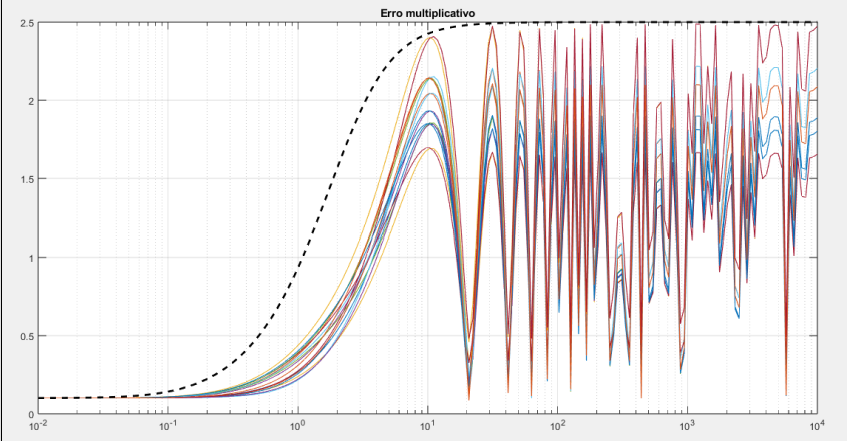
\includegraphics[width=0.82\textwidth]{figure9.png}
  \caption{Curvas de erros multiplicativos}
  \end{figure}

  \begin{figure}[H]
  \centering
  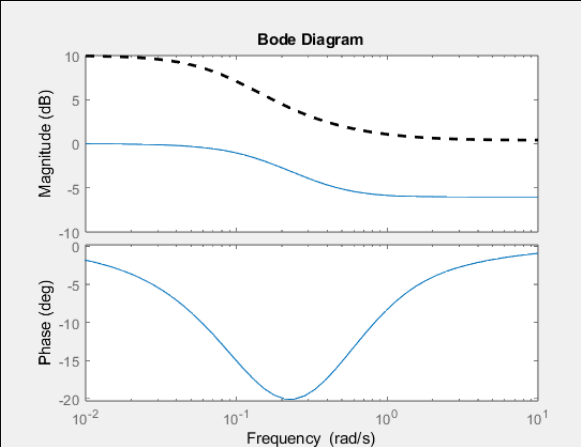
\includegraphics[width=0.82\textwidth]{figure10.png}
  \caption{Análise de Robustez }
  \end{figure}

É evidente que o nosso sistema apresenta uma robustez significativa. Isso explica porque a variação máxima do ponto de operação que ainda foi possível controlar foi muito próxima neste experimento, começando a se desviar com uma variação de 0.5 na referência de \(C_B\).

















\subsection{Preditor de Smith Filtrado}

c) Considere agora que deseja melhorar a resposta do Preditor de Smith. Utilize então um Preditor de Smith filtrado para o controle de \(C_B\). O que pode ser melhorado com este novo controle? Repita as simulações para o modelo linear e não linear. A performance é melhorada como previsto em ambos os casos? Discuta e justifique os resultados com uma análise de robustez do sistema. Encontre o controle equivalente e analise a ordem do mesmo e sua implementação por equações a diferença.\\

\begin{equation}
C_{B}(z) = \frac{(-0.04658z^2 + 0.02241z + 0.069)}{(z^2 - 1.501z + 0.543)} U(z)
\end{equation}

\begin{equation}
C_{B}(z) =  \frac{(-0.04658z^2 + 0.02241z + 0.069)}{(z-0.608)(z-0.893)} U(z)
\end{equation}

Devemos realizar o desenvolvimento de um Preditor de Smith com filtro de projeção, o qual a estrutura pode ser vista abaixo.


\begin{figure} [h]
    \centering
    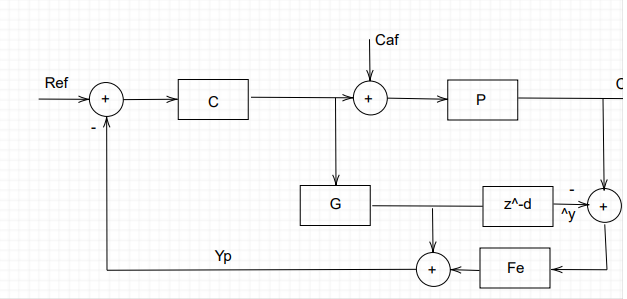
\includegraphics[width=0.8\linewidth]{image1.png}
    \caption{Diagrama de Blocos de Preditor de Smith Filtrado}
    \label{fig:enter-label}
\end{figure}

Dessa forma, é visto que podemos utilizar a estrutura do Preditor de smith projetada na questão 1 deste relatório, onde temos

\begin{equation}
C(z) = \frac{0.9928z - 0.8672}{z - 1}
\end{equation}

\begin{equation}
Fr(z) = \frac{0.1256}{0.9928z - 0.8672}
\end{equation}\\

Necessitando apenas realizar o projeto do filtro de projeção.


Para fazer o desenvolvimento de filtro de projeção temos que atender duas condições, são elas, ganho do filtro deve ser unitário e a seguinte equação deve ser atendida:

\begin{equation}
1 - Fe \cdot z^{-d} |_{(z=pzi)} = 0 
\end{equation}

Onde pz são os polos indesejados. Como temos uma planta de segunda da ordem, o filtro de projeção deve ter a seguinte estrutura:

\begin{equation}
Fe(z) = \frac{a^2z+bz+c}{(z-\lambda)^2}
\end{equation}


Vamos iniciar obtendo o valor de \(\lambda\), utilizando o tempo de assentamento desejado e a aproximação para polos reais e iguais. Para facilitar, obtemos inicialmente o polo desejado  no continuo e depois realizaremos a discretização.


Polo desejado no contínuo:

\begin{equation}
t_{(5\%)} = \frac{3}{pd} = 1.5 \xrightarrow{} pd = \frac{3}{1.5} = 2
\end{equation}

Passando para o discreto, temos:

\begin{equation}
\lambda = e^{(-pd.Ts)} = e^{(-2*0.07)} = 0.869
\end{equation}

Aplicando o filtro de projeção na primeira condição:

\begin{equation}
Fe(1) = 1 → \frac{a+b+c}{(a-\lambda)^2} = 1
\end{equation}

Obtemos a seguinte equação:

\begin{equation}
a+b+c = (1-\lambda)^2
\end{equation}

Aplicando o filtro de projeção na segunda condição:

\begin{equation}
1-Fe * z ^-d |_{z=pzi} = 0
\end{equation}

\begin{equation}
1-\frac{apz^2_i + bpz_i + c}{(pz_i + \lambda)^2} * pz^{-d}_i = 0
\end{equation}

Chegamos na seguinte equação:

\begin{equation}
a * pz^2_i + b*pz_i + c = (pz_i - \lambda)^2 * pz^d_i
\end{equation}

Como temos dois polos indesejados, vamos obter as seguintes iguais com valores dos polos indesejados. Com essas duas e mais a equação obtida pela primeira condição obtemos o seguinte sistema de equações.

\begin{equation}
a + b + c = (1 - \lambda)^2
\end{equation}
\begin{equation}
a * pz^2_1 + b * pz_1 + c = (pz_1 - \lambda)^2 * pz^d_1
\end{equation}
\begin{equation}
a * pz^2_2 + b * pz_2 + c = (pz_2 - \lambda)^2 * pz^d_2
\end{equation}\\


Tendo os valores para \(pz_1 = 0.608\), \(pz_2 = 0.893\), \(d = 43\), \(\lambda = 0.869\). Temos:


\begin{equation}
a + b + c = (1 - 0.869)^2
\end{equation}
\begin{equation}
a * (0.608)^2 + b * 0.608  + c = (0.608 - 0.869)^2 * 0.608^{43}
\end{equation}
\begin{equation}
a * (0.893)^2 + b * 0.893  + c = (0.893 - 0.869)^2 * 0.893^{43}
\end{equation}\\

Resolvendo o sistema de equações acima, obtemos os seguintes valores para os parametros do filtro de projeção

\begin{equation}
a =  0.409141
\end{equation}
\begin{equation}
b = -0.61412
\end{equation}
\begin{equation}
c = 0.222141
\end{equation}\\

Dessa forma, obtemos o seguinte filtro de projeção:\\

\begin{equation}
Fe(z) = \frac{0.409141z^2 - 0.61412z + 0.222141}{(z-0.869)^2}
\end{equation}
\begin{equation}
Fe(z) = \frac{0.409141z^2 - 0.61412z + 0.222141}{z^2 - 1.738 + 0.755}
\end{equation}\\

Agora iremos analisar o comportamento do sistema linear com o Preditor de Smith Filtrado, adicionando o filtro de projeção na estrutura do Preditor de Smith, obtemos:

\begin{figure}[h]
    \centering
    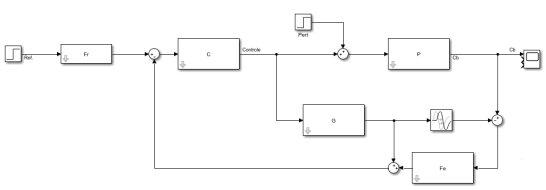
\includegraphics[width=0.9\linewidth]{image2.png}
    \caption{Estrutura Preditor de Smith Filtrado}
    \label{fig:enter-label}
\end{figure}

Contudo, para que possamos implementar o filtro desenvolvido, temos que alterar a estrutura do Preditor de Smith afim de obter uma equivalente estável. Dessa forma, chegamos no seguinte Preditor de Smith filtrado equivalente estável e implementável.

\begin{figure}[H]
    \centering
    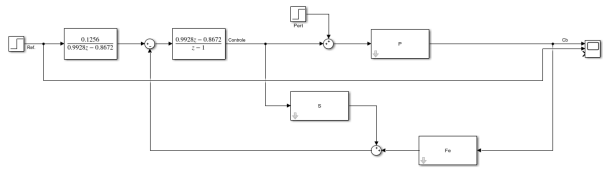
\includegraphics[width=0.9\linewidth]{image3.png}
    \caption{Estrutura Preditor de Smith Filtrado Implementavel (Modelo linear)}
    \label{fig:enter-label}
\end{figure}

Onde:

\begin{equation}
S = G(z)*(1-Fe(z)z^-d)
\end{equation}
\begin{equation}
P = G(z)*z^-d
\end{equation}

Dessa forma, obtemos a seguinte resposta a mudanças do tipo degrau na referencia:

\begin{figure}[H]
    \centering
    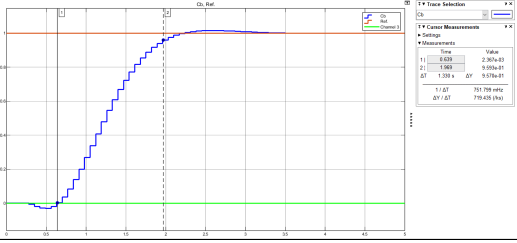
\includegraphics[width=0.9\linewidth]{image4.png}
    \caption{Respostas P.S.F a mudanças de degrau na referência (Modelo linear)}
    \label{fig:enter-label}
\end{figure}

Agora, obtemos a seguinte resposta a mudanças do tipo degrau na perturbação:

\begin{figure}[H]
    \centering
    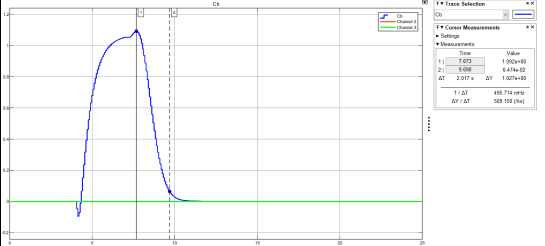
\includegraphics[width=0.9\linewidth]{image5.png}
    \caption{Respostas P.S.F a mudanças de degrau na perturbação (Modelo linear)}
    \label{fig:enter-label}
\end{figure}

Assim, para o sistema não linear temos a seguinte estrutura:

\begin{figure}[H]
    \centering
    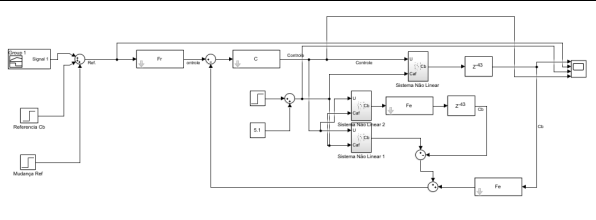
\includegraphics[width=0.9\linewidth]{image6.png}
    \caption{Estrutura Preditor de Smith Filtrado Implementavel (Modelo não linear)}
    \label{fig:enter-label}
\end{figure}

Onde, obtemos a seguinte resposta a mudanças do tipo degrau na referencia:

\begin{figure} [H]
    \centering
    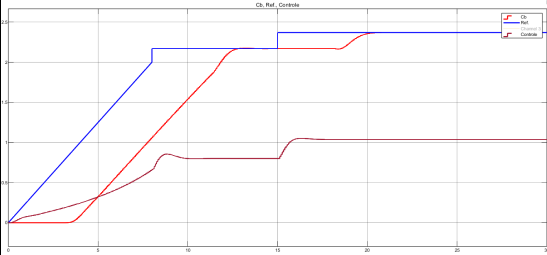
\includegraphics[width=0.9\linewidth]{image7.png}
    \caption{Respostas P.S.F a mudanças de degrau na referência (Modelo não linear)}
    \label{fig:enter-label}
\end{figure}

Neste caso, obtemos um tempo de assentamento de 1.52 minutos, oque visto pelo grupo é aceitavel.

E tambem a seguinte resposta para mudanças do tipo degrau na perturbação:

\begin{figure} [H]
    \centering
    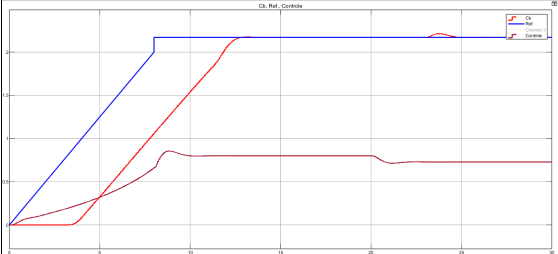
\includegraphics[width=0.9\linewidth]{image8.png}
    \caption{Respostas P.S.F a mudanças de degrau na perturbação (Modelo não linear)}
    \label{fig:enter-label}
\end{figure}

Para mudanças do tipo degrau, obtemos o tempo de assentamento de
aproximadamente um minuto.


Para estudar a robustez do sistema utilizamos o código anterior e multiplicamos \(\frac{Y}{R}\) pelo filtro \(\mathcal{F}_e\) e obtivemos o seguinte gráfico:


\begin{figure} [H]
    \centering
    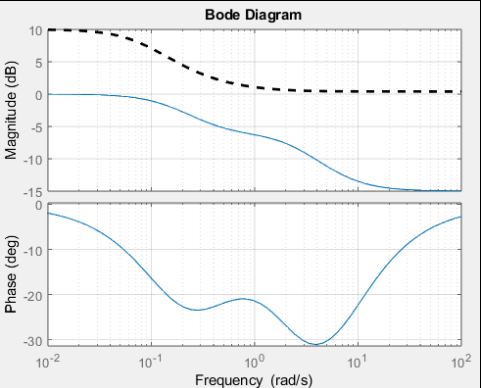
\includegraphics[width=0.6\linewidth]{image9.png}
    \caption{Análise de Robustez P.S Filtrado}
    \label{fig:enter-label}
\end{figure}

Como podemos ver, o uso do filtro piorou um pouco a robustez do sistema no caso linear, tordando-o mais sucetivel a mudanças e variações em torno do ponto de operação.

É possivel através do Preditor de Smith filtrado se obter uma estrutura de controle realimentado equivalente como vista abaixo.

\begin{figure} [H]
    \centering
    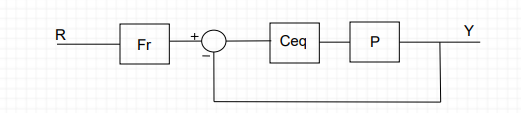
\includegraphics[width=0.9\linewidth]{image10.png}
    \caption{Diagrama de Blocos Preditor de Smith Filtrado}
    \label{fig:enter-label}
\end{figure}

Onde o controlador equivalente é dado da seguinte forma:

\begin{equation} 
Ceq = \frac{Nc*Fe}{Dc+NcNg*Dx} 
\end{equation}\\
Onde:\\
\begin{equation} 
Dx = \frac{1-Fe*e^{-Ls}}{Dg}
\end{equation}\\

Utilizando o matlab, chegamos no seguinte controlador equivalente:

\begin{figure} [H]
    \centering
    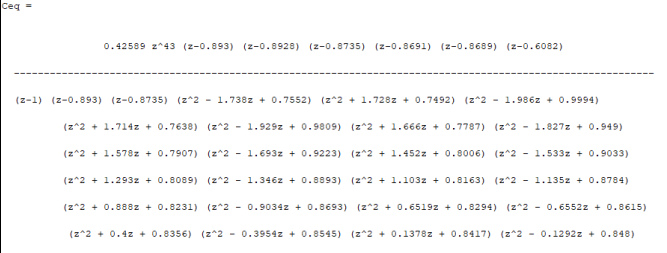
\includegraphics[width=0.9\linewidth]{image11.png}
    \caption{Controlador equivalente do P.S.F}
    \label{fig:enter-label}
\end{figure}

Como podemos observar o controlador equivalente possui uma ordem bastante elevada, o que dificultaria bastante a sua implementação, portanto, o grupo atribui ao preditor de smith o titulo de uma opção mais adequada para a solução do problema.


\end{document}